%%%%%%%%%%%%%%%%%%%%%%%%%%%%%%%%%%%%%%%%%
% Journal Article
% LaTeX Template
% Version 1.3 (9/9/13)
%
% This template has been downloaded from:
% http://www.LaTeXTemplates.com
%
% Original author:
% Frits Wenneker (http://www.howtotex.com)
%
% License:
% CC BY-NC-SA 3.0 (http://creativecommons.org/licenses/by-nc-sa/3.0/)
%
%%%%%%%%%%%%%%%%%%%%%%%%%%%%%%%%%%%%%%%%%

%----------------------------------------------------------------------------------------
%	PACKAGES AND OTHER DOCUMENT CONFIGURATIONS
%----------------------------------------------------------------------------------------

\documentclass[fancy]{article}

\usepackage{lipsum} % Package to generate dummy text throughout this template

\usepackage[sc]{mathpazo} % Use the Palatino font
\usepackage[T1]{fontenc} % Use 8-bit encoding that has 256 glyphs
\linespread{1.05} % Line spacing - Palatino needs more space between lines
\usepackage{microtype} % Slightly tweak font spacing for aesthetics

\usepackage[hmarginratio=1:1,top=32mm,columnsep=20pt]{geometry} % Document margins
\usepackage{multicol} % Used for the two-column layout of the document
\usepackage[hang, small,labelfont=bf,up,textfont=it,up]{caption} % Custom captions under/above floats in tables or figures
\usepackage{booktabs} % Horizontal rules in tables
\usepackage{float} % Required for tables and figures in the multi-column environment - they need to be placed in specific locations with the [H] (e.g. \begin{table}[H])
\usepackage{hyperref} % For hyperlinks in the PDF
\usepackage{authblk}
\usepackage{amsmath}
\usepackage{csvsimple}
\newcommand{\resultcsv}{results.csv}
\usepackage{pgfplotstable}

\usepackage{color}

\definecolor{pblue}{rgb}{0.13,0.13,1}
\definecolor{pgreen}{rgb}{0,0.5,0}
\definecolor{pred}{rgb}{0.9,0,0}
\definecolor{pgrey}{rgb}{0.46,0.45,0.48}



\usepackage{listings}
\lstset{language=C++,
  showspaces=false,
  showtabs=false,
  breaklines=true,
  showstringspaces=false,
  breakatwhitespace=true,
  commentstyle=\color{pgreen},
  keywordstyle=\color{pblue},
  stringstyle=\color{pred},
  basicstyle=\ttfamily,
  moredelim=[il][\textcolor{pgrey}]{$$},
  frame = single,
  numbers=left, 
  numberstyle=\small,
  belowskip=3em,
  aboveskip=2em,
  moredelim=[is][\textcolor{pgrey}]{\%\%}{\%\%}
}

\usepackage[T1]{fontenc}
\usepackage[scaled]{beramono}
\newcommand\Small{\fontsize{9}{9.2}\selectfont}
\newcommand*\LSTfont{\Small\ttfamily\SetTracking{encoding=*}{-60}\lsstyle}

\usepackage{lipsum}
\newenvironment{Figure}
  {\vspace{5mm}\par\medskip\noindent\minipage{\linewidth}}
  {\endminipage\par\medskip\vspace{5mm}}


\usepackage{lettrine} % The lettrine is the first enlarged letter at the beginning of the text
\usepackage{paralist} % Used for the compactitem environment which makes bullet points with less space between them

\usepackage{graphicx}

\usepackage{abstract} % Allows abstract customization
\renewcommand{\abstractnamefont}{\normalfont\bfseries} % Set the "Abstract" text to bold
\renewcommand{\abstracttextfont}{\normalfont\small\itshape} % Set the abstract itself to small italic text

\everymath{\displaystyle}

\usepackage{titlesec} % Allows customization of titles
\renewcommand\thesection{\Roman{section}} % Roman numerals for the sections
\renewcommand\thesubsection{\Roman{subsection}} % Roman numerals for subsections
\titleformat{\section}[block]{\large\scshape\centering}{\thesection.}{1em}{} % Change the look of the section titles
\titleformat{\subsection}[block]{\large}{\thesubsection.}{1em}{} % Change the look of the section titles

\usepackage{fancyhdr} % Headers and footers
\pagestyle{fancy} % All pages have headers and footers
\fancyhead{} % Blank out the default header
\fancyfoot{} % Blank out the default footer
\fancyhead[C]{VU Algorithmics $\bullet$ Winter Semester 2014/15}
% Custom header text
\fancyfoot[RO,LE]{\thepage} % Custom footer text

%----------------------------------------------------------------------------------------
%	TITLE SECTION
%----------------------------------------------------------------------------------------

\title{\vspace{-15mm}Experimental report on \vspace{5mm} \\
\fontsize{24pt}{10pt}\selectfont\textbf{Time-Constrained Bipartite Vehicle Routing Problem}}
% Article title

\author[1]{Michael Hartl\thanks{A.A@university.edu}}
\author[1]{Soroosh Mortezapoor\thanks{1225049}}
\affil[1]{Vienna University of Technology}

\renewcommand\Authands{ and }

\date{}

%----------------------------------------------------------------------------------------

\begin{document}


\maketitle % Insert title
\begin{abstract}
In this report, it is tried to solve a problem called Time-Constrained Bipartite
Vehicle Routing Problem (TCBVRP) by mixed integer linear programing through
formulating and implementing in C++ for CPLEX solver and eventually a brief
description on utilized algorithms and selected approach along with
some experimental results is presented.
\end{abstract}


\thispagestyle{fancy} % All pages have headers and footers

%----------------------------------------------------------------------------------------
%	ABSTRACT
%----------------------------------------------------------------------------------------





%----------------------------------------------------------------------------------------
%	ARTICLE CONTENTS
%----------------------------------------------------------------------------------------


\smallskip
\noindent \textbf{Keywords.} Integer Programming, CPLEX, ILOG, Vehicle Routing,
Algorithms




\section{Introduction}
The main task which is tried to be achieved in this experiment and project
is to find an optimal solution for a Time-Constrained Bipartite Vehicle Routing
Problem, known as TCBVRP hereafter defined by following
characteristics:

Given an asymmetric weighted Graph $G=(N,A)$ where $N$ comprises three
kind of nodes, demand nodes (D), supply nodes (S) and a single depot and the weight of
arcs corresponds to the travel time from their tales to their heads utilizing
maximum $m$ available vehicles, maximum $m$ tours is demanded having the lowest cost
among all possible solutions. Besides, the length of each tour cannot exceed a
certain amount defined by inputs.

In order to find such an optimal solution there are some restrictions that
should be taken into consideration which come following and will be referred to
later in this report.

Here are these restrictions:

\begin{enumerate}
  \item Each demand node is visited exactly once
  \item Each supply node is visited at most once
  \item Each tour starts and ends at the depot
  \item The first visited node in each tour is a supply node
  \item The last visited node in each tour must always be a demand
node.
\item Only arcs between different types of nodes are allowed
\item The total time of a tour shall not exceed a threshold T
\end{enumerate}

Figure \ref{fig:vis} illustrates one of the input instances and all
possible connections to use among the nodes.\footnote{The graph is visualized by
Networkx\cite{hagberg2004networkx} and PyPlot libraries in Python 2.7}. Gray $0$ node shows the depot while green nodes indicate supply
nodes $S$ and red nodes present demand nodes $D$.

\begin{figure}[H]
  \centering
    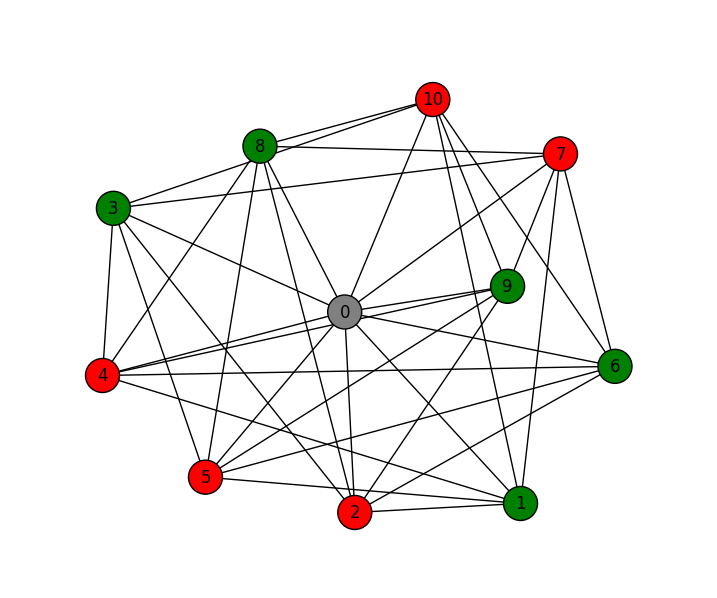
\includegraphics[width=0.5\textwidth]{./figures/instance1.png}
    
  \caption{\label{fig:vis} Visualisation of the first input instance. Gray,
  green and red nodes are the depot, supply nodes and demand nodes
  respectively.}
  
\end{figure}

In the next section, formulation and implementation every single one of these
constraints is discussed and shown.

\section{Formulation}
Moving toward the ultimate goal of finding an optimal solution for the problem
stated before, the first step is to formulate this problem is a way solvable by
integer programming \cite{garfinkel1972integer}. Subsequently these formulae can be easily structured
and implemented such that available integer programming solvers can be utilized to
find our required answer. Here as suggested by course instructors, IBM ILOG
CPLEX Solver \cite{cplex2009v12}
is used to find the proper answer to a mixed integer linear program created and
formulated out of requirements of mentioned problem.

Short after formulating the problem, the implementation is given based on three
different flow control methods, single commodity flows, multi commodity flows
and Miller-Tucker-Zemlin subtour elimination constraints which are used to
eliminate subtours from our solutions.

Starting with the standard TSP \cite{miller1960integer} formulation, we have to adjust it a
little to account for the extra properties in TCBVRP. Our basic variables are not
indexed $x_{ij}$ as in two dimensions, but $x_{ijk}$ where $k$ is the number
of the tour. So we need $n*n*m$ variables instead of just $n*n$, and $x_{ijk} \in \{0,1\}$
indicates whether the arch from $i$ to $j$ was taken in tour $k$ (then $x_{ijk} = 1$) or
not ($x_{ijk} = 0$).

After declaring the variables, the next thing which is mandatory is an objective function 
that can be optimized. Here it is proposed to try to minimize following function as our
objective function:

\begin{equation}
\mbox{minimize }\sum_{k = 1}^{m} \sum_{i = 0}^{n} \sum_{j = 0}^{n} c_{ij} x_{ijk}
\end{equation}

Where $c_{ij}$ designates the cost of the connection $ij$.

Now since the objective function is declared, so the constraint must be defined
as well. Let's start with the requirements listed before and formulate them one
by one.

The basic constraints are the same for all three formulations. $D$ denotes the
set of demand nodes, $S$ the set of supply nodes. If not otherwise designated,
then $i, j \in N$ and $k \in M$. We designate the depot as node $0$.

\begin{description}
  \item[Each demand node is visited exactly once.]
    \begin{equation}
      \forall j \in D. \sum_{i,i \neq j, k} x_{ijk} = 1
    \end{equation}
  \item[Each supply node is visited at most once.]
    \begin{equation}
      \forall j \in S. \sum_{i,i \neq j, k} x_{ijk} \leq 1
    \end{equation}
  \item[Each node is left as often as it is visited.]
    \begin{equation}
      \forall j \in N. \forall k \in M. \sum_{i,i \neq j} x_{ijk} = \sum_{l \in N, l \neq j} x_{jlk}
    \end{equation}
    This formulation also ensures that a certain node is visited
    and left in the same tour. If we had just mimicked the two 
    preceding constraints for outgoing connections as well,
    then it would be possible to visit a node in one tour
    and leave it in the other.        
  \item[The depot is visited once in each tour.]
    \begin{equation}
      \forall k. \sum_{i} x_{i,0,k} = 1
    \end{equation}
  \item[Each connection is either taken or not.]
    \begin{equation}
        \forall i,j \in N. \forall k \in M. \begin{cases} 
          &x_{ijk} \in \{0,1\} \mbox{ iff. $ij$ allowed} \\
          &x_{ijk} = 0 \mbox{ otherwise}
      \end{cases}
    \end{equation}
    Allowed connections are those allowed in TCBVRP, i.e.
    \begin{itemize}
      \item $Supply \rightarrow Demand$
      \item $Demand \rightarrow Supply$
      \item $Demand \rightarrow Depot$
      \item $Depot \rightarrow Supply$
      \item $Depot \rightarrow Depot$
    \end{itemize}

    Note that $Depot \rightarrow Depot$ is allowed, thus making empty tours possible. 
    This means that there is intentionally no $i \neq j$  property in the above 
    formula while it is present in the formulation
    of the original TSP problem. All other self-connections are forbidden by the 
    $allowed$ rule above though.

  \item[No subtour can be longer than $T$.]
    \begin{equation}
      \forall k. \sum_{i} \sum_{j} x_{ijk} c_{ij} \leq T
    \end{equation}
\end{description}

\subsection{Single Commodity Flow (SCF)}

We need the additional constraints in SCF, MCF and MTZ to avoid subtours. The idea n SCF is
to send out some commodity from the depot and have each reached node subtract one. Thus, a 
subtour which does not include the depot is not possible because no flow would be coming in
and therefore the nodes inside the subtour would have negative flow, which is forbidden.

We introduce a new set of variables $f_{ijk}$, corresponding to $x_{ijk}$ describing the units
of flow over a certain arch $ij$ in a tour $k$. If $x_{ijk} = 0$, then $f_{ijk} = 0$, too.

\begin{description}
  \item[The depot sends out $|D|$ units of flow.] $D$ here is the set of demand nodes. We do 
  not need to send out flow for supply nodes because they do not necessarily have to be
  reached at all, and they cannot form subtours on their own because it's not allowed to 
  go from a supply node to anywhere but a demand node.
     \begin{equation}
       \sum_{j>0,k} f_{0jk} = D
     \end{equation}

  \item[A node is either reached in a certain tour or not.]
     Compared to the standard TSP problem we have to deal with a complication here: A node which 
     is not reached in a certain tour does not get any flow and therefore cannot subtract one,
     so we have to distinguish between reached nodes and unreached nodes, giving rise to a new
     variable $r_{jk} \in \{0,1\}$ and the following constraint.
     \begin{equation}
        \forall j>0. \forall i \neq j. \forall k. r_{jk} \geq x_{ijk}
     \end{equation}
     This ensures that $r_{jk}$ is $1$ if $j$ is reached, but it cannot also be $1$ if it unreached,
     because this would mean that $j$ would be forced to subtract a flow unit which it cannot
     do because there would be no incoming flow.

  \item[A demand node subtracts a unit of flow if it reached in a tour, and passes it on unmodified
        otherwise.] We can now formulate this crucial property.
  \begin{equation}
        \forall j>0 \in D. \forall k. \sum_{i \neq j} f_{ijk} = \sum_{l \neq j \in N} f_{jlk} = r_{jk}
  \end{equation}

  \item[Any other node passes on flow unmodified.]
  \begin{equation}
        \forall j>0, j \in N \setminus D. \forall k. \sum_{i \neq j} f_{ijk} = \sum_{l \neq j \in N} f_{jlk} = 0
  \end{equation}

  \item[flow is at most $|D|$ or $0$] 

  If an arch is not taken, then the flow along it must be zero. Otherwise it may be positive, but 
  not more than $|D|$.

  \begin{equation}
        \forall i. \forall j \neq i. \forall k. 0 \leq f_{ijk} \leq |D| x_{ijk}
  \end{equation}
\end{description}

\subsection{Multi Commodity Flow (MCF)}

This is very similar to SCF, but we need $|D|$ times more variables, because we send out $|D|$ commodities, and only one unit of each. Thus, our $f_{ijk}$ variables turn into $f_{ijkc}$, where $c$ is the index of a demand node corresponding to a commodity.

\begin{description}
  \item[The depot sends out $1$ unit of flow per demand node.]
     \begin{equation}
       \forall c \in D. \sum_{j>0,k} f_{0jkc} = 1
     \end{equation}

  \item[There is no flow going back to the depot.]
     \begin{equation}
       \forall c \in D. \sum_{i>0,k} f_{i0kc} = 0
     \end{equation}

  \item[A node is either reached in a certain tour or not.]
     \begin{equation}
        \forall j>0. \forall i \neq j. \forall k. r_{jk} \geq x_{ijk}
     \end{equation}

  \item[A demand node subtracts a unit of flow if it reached in a tour, and passes it on unmodified
        otherwise.] We can now formulate this crucial property.
  \begin{equation}
        \forall j>0 \in D. \forall k. \sum_{i \neq j} f_{ijk} = \sum_{l \neq j \in N} f_{jlk} = r_{jk}
  \end{equation}

  \item[Any other node passes on flow unmodified.]
  \begin{equation}
        \forall j>0, j \in N \setminus D. \forall k. \sum_{i \neq j} f_{ijk} = \sum_{l \neq j \in N} f_{jlk} = 0
  \end{equation}

  \item[flow is at most $|D|$ or $0$] 

  If an arch is not taken, then the flow along it must be zero. Otherwise it may be positive, but 
  not more than $|D|$.

  \begin{equation}
        \forall i. \forall j \neq i. \forall k. 0 \leq f_{ijk} \leq |D| x_{ijk}
  \end{equation}


\end{description}


\section{Implementations}
In this section, each part is described in terms of implementation. All codes
are in {\it C++} language using CPLEX Solver.
The first important part would be the objective function.

As it is shown in the code above, there is a decision variable called
\texttt{ max } used to eliminate all unwilling cases from possible selected
possibilities. For instance this variable is \texttt{ 1 } for a connection from
a node $D$ to a node $S$ or vice versa but \texttt{ 0 } for a connection between
two nodes with the same type since we don't want to have any direct connection
from a $S$ node to another $S$ node or any $D$ node to another $D$ node.

Moving, we get to the constraints. In order to keep this report short enough,
only one samples of how the constraints are implemented, is presented and the
rest lie in the code which is enclosed and fully documented and can be found at
its GitHub repository\footnote{\url{https://github.com/firefrorefiddle/ag_ex}}.
As an instance, we know that sum of incoming connections for each node should
be exactly equal to the sum of outgoing connections from that node. This
constraint is implemented as shown in Appendix\ref{app:app01}.

The other important part of the implementation is eliminating subtours from
results. Such subtours are not connected to the node \texttt{depot}. Thus it is
decided to emit the initial flow from the node \texttt{depot} to all tours
simultaneously and evaluate the inflow of the  \texttt{depot} at the end. On the
other hand, by characteristics of the problem we know that only one of the nodes
$D$ or $S$ alone cannot appear in a path and they come consecutively. Thus in
the implementation only half of the nodes in a tour which are $D$ nodes are
considered as consumers of flow and therefore $\frac{l_k}{2}-1$, $l_k$ denoting
the number of participant nodes in each tour, is the flow amount emitted from
the \texttt{depot} for that tour.
Finally:

\begin{center}
$\sum_{k=0}^{m}{\frac{l_k}{2}-1} = |D| - 1$
\end{center}

\subsection{Single commodity flows}

So for {\it single commodity flows} we have counted all connected $D$ nodes to
the \texttt{depot} over all tours and it must be exactly $|D|$ nodes in whole
system.

A simplified version of the implementation of this part is demonstrated in
Appendix\ref{app:app02}.

\subsection{Multi commodity flows}


Multi commodity flows is considerable similar to single commodity flows. The
only difference is that this time, \texttt{ depot } sends out only $p$ flows out
but $n$ times, in our case $\#D$ times, and expects $p-1$ back. Consequently,
wrapping the code used for single commodity flows in a loop which iterates $\#D$
times and deciding over \texttt{(sumDepotOut - sumDepotIn) == 1} results in
elimination of subtours using multi commodity flows.

\subsection{Miller-Tucker-Zemlin subtour elimination constraints}


\section{Experimental Results}
\begin{filecontents*}{results.csv}
\end{filecontents*}

\begin{tabular}{l|l}%
    \bfseries SCF & \bfseries MCF% specify table head
    \csvreader[head to column names]{Basket_ball.csv}{}% use head of csv as column names
    {\\\hline\csvcoli&\csvcolii}% specify your coloumns here
\end{tabular}

\section{Conclusion}
Using SCF and MCF we were able to solve most problem instances of up to 30 nodes.
However SCF was able still to solve one instance with 60 nodes. Nonetheless,
those with 60, 90, 120 or 180 nodes were out of reach.
Compared to two other algorithms, MTZ showed a rather poor performance and
it came up with some results in reasonable time only for the smallest
instances with 10 nodes. Although SCF and MCF seem very similar in comparison
of their results, SCF tends to perform slightly better.

Finally, there seems to be a long way to traverse toward optimizing the
implementation of these algorithms provided that applying them on a real application domain is
desired.



%----------------------------------------------------------------------------------------
%	REFERENCE LIST
%----------------------------------------------------------------------------------------
\bibliographystyle{plain}
\bibliography{references} 

%----------------------------------------------------------------------------------------


\end{document}
